	The term "generaliZability" is used widely in literature, despite rarely being particularly well defined. Often, generalizability refers merely to the state of a predictor as "not overfitted". In other words, that it maintains sufficient performance across the training, validation, and test-sets. This, however, typically neglects the more salient aspects of the performance of the pipeline; namely how it behaves when deployed in practical settings, on data that may be distributed differently from the training dataset. Consider for instance the problem of detecting and classifying traffic signs. Though it is relatively trivial to achieve decent performance on such a task when training and evaluating on one specific dataset, it is another matter entirely to make sure the resulting predictors are robust to any and all forms of variability one might expect to see when deployed in a practical setting. If the training data was for instance collected from a region with a dry, temperate climate, it might not come as a surprise that it will not perform as well when deployed in an area prone to snowfall, fog, or generally low visibility. Of course, this could be mitigated by ensuring that the training data contains samples from a wide variety of climates, but this really only affects the robustness of the pipeline to differing climates. It does not necessarily ensure that the resulting predictors learn to ignore weather effects entirely, and as such it may nonetheless fail if it encounters something it has not been explicitly trained on. This is made especially evident in the study of black-box adversarial attacks: %examples ...
	        
	In other words, merely being robust to a limited class of perturbations or variability is not sufficient to deem a pipeline as generalizable. The pipeline must not merely learn to be right, but right for the right reasons. If this is achieved, robustness to distributional shifts follows. The system outlined above should in other words not only be robust to snow or rain or fog, but to be able to ignore the effects thereof entirely. A perfectly generalizable pipeline shouuld return a weather-invariant predictor every time, and for that matter maintain invariance to any and all non-destructive distributional shifts. 
	        
	The term generalizability will as such in this thesis refer to the ability to infer the right inductive biases from an incomplete dataset. This is as opposed to robustness, which denotes the ability of a pipeline to maintain its performance across certain distributional shifts. Generalizability is as a consequence not as much of a measurable quantity as much as it is an emergent property of a well-designed pipeline. 
	        
	This section will explore the concept of generalizability in further detail. It will outline how typical deep learning-based systems aim to achieve generalizability, why it nonetheless often fails to do so, and how one can analyse such generalizability failure.
	
			Naturally, however, real-world data is rarely neat enough for it to consistently abide by the iid assumption. Commonly encountered variation in real world data such as variable lighting conditions, class imbalance, image corruptions, noise, or other more subtle forms of distributional shift all result in structural misalignment of the training and deployment distributions (citation). Ideally, predictors should be robust to these sorts of changes, however evidently this is in not guaranteed by ERM (citation). ERM simply guarantees an iid-optimal predictor. While the difference is subtle, it is worth reemphasizing: empirical risk minimization only generalizes to data which is more or less identically distributed to the training data. Differently distributed or otherwise perturbed data, even that which is near imperceptible or at any rate inconsequentially different to the human eye, violates the iid assumption, and can as such not be expected to be classified correctly given a predictor trained via ERM. 
	
	To mitigate this, one could simply add more data to the pipeline through augmentation, or simply collecting more training data. This will lead to a better approximation of the true risk. This does not, however, solve the problem. The variability of the real world is not, unfortunately, easy to model merely through augmentations, and collecting sufficient data to cover every potential source of natural variability is infeasible, especially in medical domains. 
	%link this
	Consider for example a machine-learning pipeline wherein a model is trained to classify cows and camels. The dataset consists of cows, pictured in grass fields and pastures, and camels, pictured in deserts. To be generous, let us assume that we have sufficient quantities of data to ensure that the pipeline is perfectly invariant to the pose of the respective animals, to lighting conditions, geometric transforms, etc. One may then expect that the pipeline correctly learns to classify the two, and attains high accuracies, and indeed when evaluated on iid data, this would be entirely correct. However, what would then happen if one such predictor encountered a cow in the desert and a camel in a grass pasture? This constitutes a distributional shift, and as such we cannot expect reliable performance as detailed in \ref{erm}. Naturally, the predictor may have learned just fine exactly what constitutes a cow and a camel, but it might just as easily learned to associate deserts with camels and pastures with cows. And from a data perspective, both are equally correct interpretations. The immediate response to this may be to simply add some pictures with more varied backgrounds, but this once again would only serve to make the pipeline more robust to backgrounds. it would not guarantee that the pipeline learns the right inductive biases. The predictor may then for example instead learn that cows typically are black and white and camels usually beige, and then fail when it encounters a brown cow. One could keep adding more and more data, but there is not really any way of knowing when the pipeline is well enough specified by the data such that it starts returning predictors with the desired inductive biases. There are in simpler terms several "correct" interpretations of what separates the classes from a purely data-based perspective, each with their own inductive biases. There are as a consequence not just one risk-minimizing predictor, but a whole family of them. This is referred to as underspecification \cite{damour2020underspecification}.
	
	
		\subsubsection{Overfitting and underfitting}
	Overfitting and underfitting are perhaps the two most well-understood instances of generalisation failure. In simple terms, underfitting occurs when the span of the hypothesis space is insufficient to adequately model the relationships the model is intended to capture. Simple linear regression would, for instance, always fail to produce a generalisable predictotor of non-linear relationships between its input variables. Similarily, a neural network may be too shallow or too short, in which case the pipeline can never, even given infinite data and an optimal optimization process, find \(f\), since it simply does not exist in \(\mathcal{H}\) This is of course a fairly trivial problem to solve: simply increase the depth and/or width  of the model. And indeed, this is principally the reason why deep learning networks have proven to be superior to its more simple counterparts.
	

	Generalization failure is then in this case and by this line of reasoning entirely dependent on the structural misalignment and distributional shift corresponding to the change in imaging techniques as opposed to any erroneous logic in the pipeline itself. Ideally, the pipeline should of course detect patterns that generalize well regardless of lighting conditions, but it is not reasonable to expect the pipeline to draw this conclusion autonomously. Instead, the pipeline has to be "told" to keep this invariance in mind during training a priori. If some hypothetical change to the pipeline were to manage to induce this invariance, the structural misalignment between the dataset would no longer be an issue, ceteris paribus.

	The behavior that violations of assumptions \ref{underfit} and \ref{overfit} is well understood and fairly easy to detect, corresponding to underfitting and overfitting respectively, but violations of the remaining assumptions result in more subtle forms of generalization failure. 
		
	The general consensus is that generalization
	failure can in broad strokes be attributed to either underspecification or structural misalignment. The following sections will attempt to summarize and synthesize the analyses within the literature, and connect each of the generalization
	failure modes they identify to the above violations.

	In broad strokes, the generalisation failure modes identified in the literature can be categorized as belonging to one of the following phenomena:
		\begin{itemize}
			\item Pareidolia
			\item Underspecification
			\item Causal agnosticism 
		\end{itemize}
		
		, consider the problem of classifying images of cows and camels as the respective animals, wherein the dataset consists of images of cows in grass fields and pastures, and camels in deserts. To be generous, let us assume that we have sufficient quantities of data to ensure that the pipeline is perfectly invariant to the pose of the respective animals, to lighting conditions, geometric transforms, weather, etc. One may then expect that the pipeline correctly learns to classify the two, and attains high accuracies, and indeed when evaluated on iid data - i.e cows in fields and camels in deserts, this would be correct. However, what would then happen if one such predictor encountered a cow in the desert and a camel in a grass pasture? This, of course, constitutes a distributional shift, and as such we cannot expect the models to generalize. The predictor may have learned just fine exactly what constitutes a cow and a camel, but it might just as easily have learned to associate deserts with camels and pastures with cows. And from a purely statistical perspective, both are equally correct interpretations. From a causal perspective, however, it is of course entirely nonsensical to assume the respective animals are wholly defined by their surroundings.


		As described in earlier sections, good generalizability can only be achieved if the pipeline can reliably generate predictors that learn causally reasonable features and consequently encode robust inductive biases. Naturally, knowing what features are causal and which are confounding is an intractable problem; otherwise generalization would simply be a matter of precisely expressing the right inductive biases algorithmically, through conventional image analysis. As a result, it is instead necessary to consider what constitutes are \texit{non-robust} features, and ensure that the model does not try to leverage these features during prediction. 

		To achieve this, a model of natural variation (MNV) is constructed, which aims to encapsulate the variability one might expect to see in the domain. This model can then be leveraged to force the DNN to be robust to the space of transformations that it defines. It is of course impossible to fully encapsulate all the possible variability one may see in the wild, but that is not necessarily obligatory so long as the search space is limited to areas wherein robust features are required. The key idea here is that it is more likely that the model learns causally viable features, than spurious features that somehow nonetheless exhibit invariance to a large space of transformations. 
		
		The construction of such a model is of course not necessarily trivial. The MNV has to be non-destructive - i.e, the model should not transform the input beyond recogniton - yet it cannot be too lenient either. The model should optimally also not affect the properties of the image that correspond to causal structure. To give a simple example: a model that classifies hand-written digits should not be invariant to rotation, as the orientation of the number 6 or 9 has causal significance, and should consequently not be included in a MNV. For more complex tasks, designing this model therefore requires some supervision - if the image at any point becomes difficult to distinguish to the human eye, the augmentations are too severe. 
	
		There are also several possible approaches as to how such a model can be leveraged. In this thesis, these approaches are as follows:
		\begin{itemize}
			\item MNV as data augmentation
			\item MNV consistency training
			\item Adversarial MNV consistency training
		\end{itemize}
	
		The reasoning behind this is that consistent behaviour should be rewarded even if the model has not quite learned how to perform to an adequate standard, as this is preferable to merely learning to perform well without any regard for consistency and by extension causality.  To illustrate, consider once more the example from chapter \ref{background}, namely the problem of acheiving generalisation from narrow-band to white-light imaging datasets and vice versa. Assume that the perturbation function simply maps between the respective lighting modalities. In this case, the loss will reward the model if it predicts identical segmentations regardless of lighting conditions, even if the predictions are incorrect. The model will nevertheless be trying to leverage features which are invariant to lighting, and consequently be more generalizable than a pipeline wherein the model is permitted to be leverage lighting-dependent features.


		Overfitting occurs when the model learns patterns that are too complex to be likely to actually describe the process(es) that generate them. Once again, to give a somewhat simple example: 
		\begin{figure}[h]
			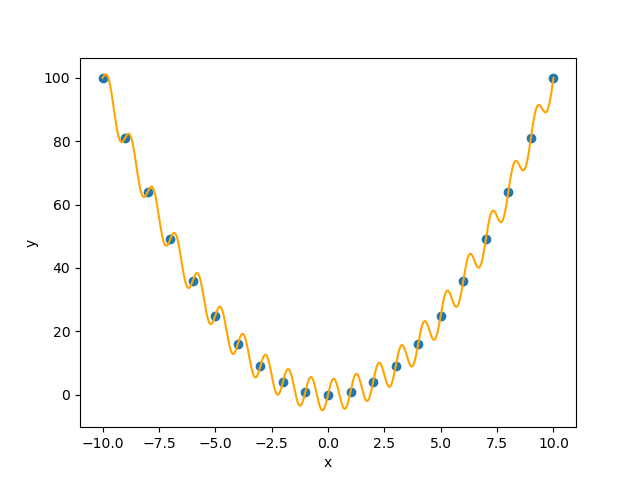
\includegraphics[width=\linewidth]{illustrations/overfit.png}
			\caption{A model with excessive capacity interpolates unneccesarily complex patterns}
			\label{Overfit example}
		\end{figure}
		The underlying function is once again \(y=x^2\). The sinusoidal pattern in the interpolated function is obviously erroneous, but this is impossible to determine with complete certainty given only a finite sampling of the underlying function. More generally, every finite sampling of any function can be interpolated as any one of an uncountably infinite set of functions. To prove this, consider the task of finding a function that fits the series \((1,4,9)\). Though ones first instinct would be to assume the pattern is described by the function \(y=x^2\), and that the next number in the sequence thus is 16, the next number can really be anything at all. Using Newton interpolation, or for that matter any arbitrary interpolation scheme, one can easily find a polynomial that fits the sequence \((1,4,9,n, n \in \mathbb{R}\). Since the set of real numbers is uncountably infinite, it follows that the space of functions that fits this new sequence also is uncountably infinite, depending on \(n\). Thus, there is an uncountably infinite number of functions that describe \(1,4,9\) as well. This of course does not only apply to extrapolating the next element in a sequence, but also any interpolating between consecutive elements. 
		Naturally, this logic also applies to neural networks. Though instead of discrete sequences, it is probability distributions that are being modelled. Just like how extrapolation and interpolation between points is ill-defined for sequences, it is ill-defined for probability distributions.
		
		Consequently, it is necessary to introduce a number of assumptions and constraints to the problem. (CLARIFY)
		
		Obviously, the minimum level of generalization one should achieve is generalization to iid data. To this end, it is necessary to incorporate an iid evaluation method, such as keeping hold-out sets, cross validation, etc. This is of course ubiquitous in modern deep learning. Moreover, it is necessary to make some assumptions regarding the simplicity - or rather, complexity - of the resulting predictor. Certain neurons should for instance not dominate the predictions, the weights should have reasonable values, etc. This is what motivates so-called regularization, whereby different methods - for instance batch normalization, drop-out, L2 loss, weight decay, etc - are used to bias the search towards areas in the loss landscape that are more credible from a perspective of model complexity. This is of course only necessary because assumptions \ref{overfit} and \ref{underspecification} do not hold. Given a perfect (or at least very well sampled) representation of the risk and consequently the loss-landscape and a perfect optimizer, the model would not overfit in any meaningful way.  

		Regularization has of course for this reason been extensively studied, and for most purposes the existing regularization techniques suffice just fine for IID data, and typically yield highly performant predictors so long as it is not subjected to any form of distributional shift. Consequently, Overfitting, though naturally still a factor that needs to be accounted for when designing deep learning pipelines, is not at fault for the generalization failure that is exhibited in modern deep learning systems.
